\chapter[Contexto da Empresa]{Contexto da Empresa}
O contexto proposto, se refere a empresa júnior Matriz - Engenharia de Energia, que é 
formada por alunos da Engenharia de Energia da Universidade de Brasilia, Campus Gama. 
O objetivo principal da Matriz é a iniciação dos alunos do curso no mercado de trabalho 
fornecendo aos clientes soluções inteligentes referentes a energia e sustentabilidade.
A empresa visa atender a demanda de residências, condomínios, empresas de médio 
e pequeno porte. 
% Inicialmente, imaginou-se que a Matriz era a fornecedora dos projetos a 
% serem trabalhados que possuiam relação com viabilidade energética e soluções sustentáveis,
% mas logo descobriu-se que a mesma só poderia fornecer pré-projetos, ela não fornecia 
% soluções. Com o passar do tempo, viu-se também que os alunos não possuem o título do CREA 
% (Conselho Regional de Engenharia e Agronomia) o que inviabiliza também que os mesmos forneçam 
% pré-projetos. No momento, a Matriz apenas realiza o contato com clientes e indica empresas 
% para a solução do problema proposto.

\section{O Problema}
Como já dito, a Matriz vêm com a proposta de ser uma Empresa Júnior que proporcione para 
os alunos de graduação uma experiência empresarial. Por ser nova, a empresa não possui 
um processo bem definido que resulte na aquisição de novos clientes. Inicialmente o que 
foi definido, consistia em investir no uso de redes sociais para difundir suas ideias, 
no estudo de mercado no que tange empresas que mais gastam energia e enviar via telefone
propostas dos serviços que a empresa disponibiliza. Feito isso, optou-se então pelo uso de
cartazes nos corredores da Faculdade do Gama (FGA), porém nenhuma das estratégias seguidas
surtiu efeito no que diz respeito a adesão de sócios e clientes.

Percebeu-se então que a Matriz não possuia uma forma facilitada de acompanhar o andamento 
do processo. Problema esse que poderia estar relacionado com a organização, gestão e 
orientação da empresa. Em um primeiro momento viu-se que a 
organização da empresa possuia grandes dificuldades em organizar os seus compromissos, 
causando desconforto nos funcionários. Sobre os recursos presentes na empresa, viu-se que 
os computadores usados, são pessoais, ou seja, cada membro usa o seu para melhor organizar-se 
da maneira que melhor o lhe convêm. 

As pessoas envolvidas, possuem pouca experiència em manusear 
sistemas de gerência de documentos, fazendo com que a documentação seja grande parte manual. Por 
possuir essa política de documentação, há grande demora quando se precisa buscar determinado 
documento, uma vez que tanto a geração como gestão dos mesmos é falha e lenta. Outro fator prejudicial, 
é a ausência de um padrão de escrita de documentos e uma adoção de um sistema que versione da melhor 
maneira. Por fim, a falta de um mecanismo que possa permitir a visualização do acompanhamento do processo
pode gerar uma maior desorganização. A ausência do mesmo, impossibilita saber o quão completa 
determinada atividade está, assim deixando os envolvidos sem saber como proceder
em alguns casos.

Os problemas e as causas encontradas ao analisar o contexto do negócio estão representados em 
um diagrama \textit{fishbone}, que pode ser visto na Figura \ref{fishbone}.
\begin{figure}[!htb]
\centering
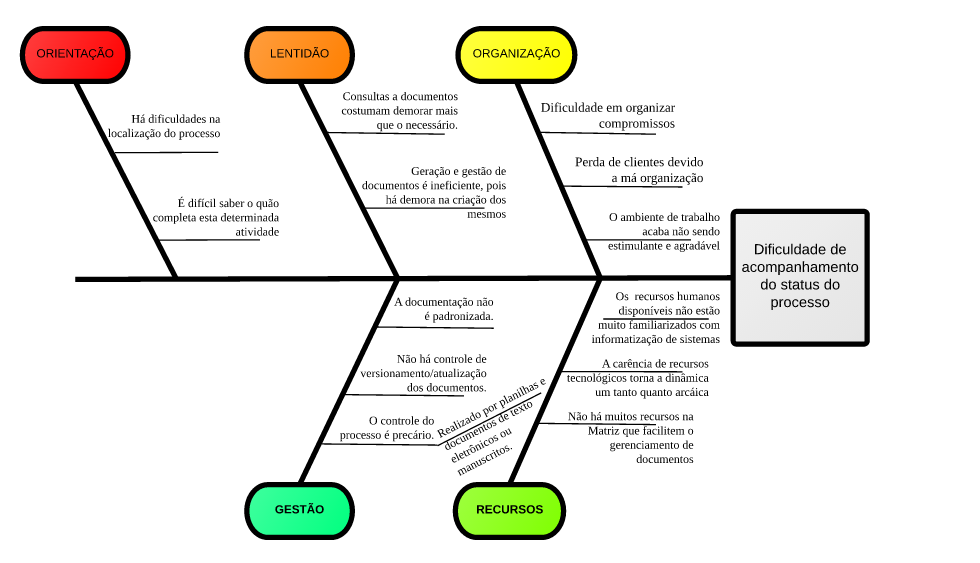
\includegraphics[scale=0.6]{figuras/fish.png}
\caption{\textit{Fishbone} obtido a partir da análise do problema}
\label{fishbone}
\end{figure}
\section{Possível Solução}
A partir deste contexto, o grupo da disciplina de Requisitos de Software, junto com um 
grupo da disciplina de Modelagem de Processos, foi encubido de criar estratégias 
criativas para obter uma maior adesão a Matriz. O problema foi identificado
usando conceitos referentes a Engenharia de Requisitos, juntos a metodologias de 
desenvolvimento adaptativas, desenhando assim um processo que consistiu desde o nível 
de análise do que de fato se necessita para reverter esse quadro, até o ponto de 
apresentar uma solução em software para o problema proposto.

Com esse mapeamento feito, espera-se que com um processo melhor desenhado e mais fácil de ser
acompanhado, a Matriz possua uma melhor abordagem e forma de lidar com clientes, e que de fato
a mesma possa captar novas pessoas para o seu melhor desenvolvimento e fornecimento de seus serviços.
